%! TeX program = lualatex
\documentclass[12pt,a4paper]{article}

\usepackage[nil]{babel}
\usepackage{unicode-math}
\usepackage[svgnames]{xcolor}
\usepackage{lmodern}
\usepackage{graphicx}
\usepackage{wrapfig}
\usepackage{float}
\usepackage{parskip}
\usepackage{hyperref}
\usepackage{listings}
\usepackage{easytable}
\usepackage{fullpage}

\definecolor{codegreen}{rgb}{0,0.6,0}
\definecolor{codegray}{rgb}{0.5,0.5,0.5}
\definecolor{codepurple}{rgb}{0.58,0,0.82}
\definecolor{backcolour}{rgb}{0.95,0.95,0.92}

\lstdefinestyle{mystyle}{
    backgroundcolor=\color{backcolour},   
    commentstyle=\color{codegreen},
    keywordstyle=\color{magenta},
    numberstyle=\tiny\color{codegray},
    stringstyle=\color{codepurple},
    basicstyle=\ttfamily\footnotesize,
    breakatwhitespace=false,         
    breaklines=true,                 
    captionpos=b,                    
    keepspaces=true,                 
    numbers=left,                    
    numbersep=5pt,                  
    showspaces=false,                
    showstringspaces=false,
    showtabs=false,                  
    tabsize=2
}


\lstset{style=mystyle}



\babelprovide[import=el, main, onchar=ids fonts]{greek} % can also do import=el-polyton
\babelprovide[import, onchar=ids fonts]{english}

\babelfont{rm}
          [Language=Default]{Liberation Sans}
\babelfont[english]{rm}
          [Language=Default]{Liberation Sans}
\babelfont{sf}
          [Language=Default]{Liberation Sans}
\babelfont{tt}
          [Language=Default]{Liberation Sans}


\setlength{\emergencystretch}{3em}

%Enter Title Here
\title{Εξόρυξη Δεδομένων και Αλγόριθμοι Μάθησης\\Εργαστηριακή Άσκηση 2022-2023}
\author{Λένος Χρίστου (ΑΜ: 1063014)\\Γρηγόρης Καπαδούκας (ΑΜ: 1072484)}

\begin{document}

\maketitle

%Insert Body Here
\setcounter{section}{-1}
\section{Αναλυτική Καταγραφή του Περιβάλλοντος Υλοποίησης}

\subsection{Καταγραφή Βιβλιοθηκών που Χρησιμοποιήθηκαν}
Για να υλοποιήσουμε την εργασία χρησιμοποιήσαμε γλώσσα προγραμματισμού\\ Python, όπως ζητείται στην εκφώνηση, με τις εξής κύριες βιβλιοθήκες:

\begin{itemize}
    \item Matplotlib
    \item Numpy
    \item Pandas
    \item Scipy
    \item Seaborn
    \item Scikit-learn
    \item Jupytext (για τη προαιρετική χρήση Jupyter Notebook)
\end{itemize}

\subsection{Αναλυτικά Βήματα για την Δημιουργία Πανομοιότυπου Περιβάλλοντος Υλοποίησης}
Παρακάτω δίνουμε αναλυτικά βήματα για την εγκατάσταση των βιβλιοθηκών σε ένα Python virtual environment, έτσι ώστε το περιβάλλον υλοποίησης να είναι πανομοιότυπο με αυτό που χρησιμοποιήσαμε εμείς:

\begin{enumerate}
    \item Εγκατάσταση του Miniconda μέσω του installer στη σελίδα:

        \textcolor{blue}{\href{https://docs.conda.io/en/latest/miniconda.html}{https://docs.conda.io/en/latest/miniconda.html}}

         Το Miniconda είναι μια δωρεάν μινιμαλιστική πλατφόρμα με cross-platform υποστήριξη που περιέχει το εργαλείο conda, με σκοπό την εύκολη δημιουργία και διαχείριση των Python virtual environments.

         Τα virtual environments αποτελούν ένα "απομονωμένο χώρο" όπου μπορούμε να εγκαταστήσουμε και να χρησιμοποιήσουμε κάποια συγκεκριμένη έκδοση της Python και βιβλιοθήκες της, χωρίς να επηρεάσουμε τυχόν εγκατάσταση της Python που βρίσκεται ήδη στο σύστημα. 

         Εναλλακτική επιλογή που μπορεί να χρησιμοποιηθεί στη θέση του Miniconda είναι το Anaconda. Το Miniconda αναφέρεται επειδή το προτιμήσαμε εμείς στην χρήση μας.

     \item Δημιουργία του conda virtual environment με αυτόματη εγκατάσταση των βιβλιοθηκών που επιθυμούμε μέσω της εκτέλεση της εξής εντολής στον φάκελο της εργασίας σε τερματικό (ή command prompt αντίστοιχα σε πλατφόρμα Windows):

         \begin{lstlisting}[language=Bash]
conda env create -f environment.yml\end{lstlisting}

         Ή άμα επιθυμείται εγκατάσταση του Jupyter Notebook ταυτόχρονα, μέσω της εντολής:

         \begin{lstlisting}[language=Bash]
conda env create -f environment-jupyter-notebook.yml\end{lstlisting}
     \item Η εγκατάσταση των βιβλιοθηκών στο virtual environment έχει ολοκληρωθεί, οπότε τώρα θα φορτώσουμε το environment με την εξής εντολή:
         \begin{lstlisting}[language=Bash]
conda activate tf\end{lstlisting}
    \item Τώρα πλέον είμαστε έτοιμοι και μπορούμε να εκτελέσουμε τον κώδικα απευθείας στο τερματικό ή μέσω του Jupyter Notebook:

        Για να εκτελέσουμε απευθείας τον κώδικα στο environment εκτελούμε απλά την εξής εντολή:
         \begin{lstlisting}[language=Bash]
python Code/<filename>.py\end{lstlisting}

        Για να εκτελέσουμε το Jupyter Notebook στο environment εκτελούμε την εξής εντολή στο τερματικό:
         \begin{lstlisting}[language=Bash]
jupyter notebook\end{lstlisting}
\end{enumerate}

\section{Υλοποίηση και Αποτελέσματα Ερωτήματος 1}

\subsection{Σύντομη Περιγραφή της Διαδικασίας Υλοποίησης}

Για την υλοποίηση του ερωτήματος αυτού, αναφέρουμε αρχικά ότι χρησιμοποιούμε την βιβλιοθήκη Pandas για το διάβασμα και την χρήστη του data.csv αρχείου με τα δεδομένα μας.

Έπειτα χρησιμοποιώντας την μέθοδο describe() του Pandas τυπώνουμε σχετικά στατιστικά στοιχεία για τα δεδομένα κάθε στήλης, πιο συγκεκριμένα τιμές για το συνολικό άθροισμα ανά στήλη (count), μέση τιμή (mean), τυπική απόκλιση (std), ελάχιστη τιμή (min), τιμές 25\%, 50\%, 75\%, και μέγιστη τιμή (max). Στις τιμές αυτές στρογγυλοποιούμε στα δύο δεκαδικά ψηφία για το τύπωμα, ώστε να είναι πιο αναγνώσιμα. 

Ακόμα τυπώνουμε μέσω for λούπας ιστογράμματα για κάθε Series του Pandas DataFrame που περιέχει τα δεδομένα του dataset, με εξαίρεση τα Series 'Country' και 'Date', για τα οποία η προβολή ιστογράμματος δεν θα μας δώσει χρήσιμη πληροφορία. Με αυτόν τον τρόπο μπορούμε να καταλάβουμε την κατανομή των δεδομένων. Για τα ιστογράμματα χρησιμοποιούμε την παράμετρο "bins = 20" με σκοπόν να κάνουμε grouping των τιμών του άξονα x σε 20 ισομεγέθη bins στο εύρος τιμών που παίρνουν οι τιμές των εισαγωγών στο Series κάθε φορά. Αυτό είναι αναγκαίο επειδή πολύ συχνά τιμές εμφανίζονται μια μόνο φορά στα δεδομένα, οπότε αν δείξουμε αυτές τις τιμές χωρίς κανένα grouping δεν θα μπορούσαμε να λάβουμε αποτελέσματα σχετικά με την κατανομή της πιθανότητας των τιμών.

Τέλος με χρήση των βιβλιοθηκών Pandas, Seaborn και Matplotlib, υπολογίζουμε αρχικά το Correlation Matrix και έπειτα κάνουμε plot το Correlation Matrix Heatmap που προκύπτει από αυτό, έτσι ώστε να εμφανίζονται οι τίτλοι των Series στους άξονες x και y και να εμφανίζονται οι τιμές του correlation που προέκυψαν στο Correlation Matrix ως κελιά στο σημείο τομής οποιονδήποτε δύο κατηγοριών. Οι τιμές για το correlation ανήκουν στο εύρος [-1,1] με 1 να σημαίνει πλήρη συσχέτιση, 0 να σημαίνει καμία συσχέτιση και -1 να σημαίνει πλήρη αρνητική συσχέτιση (πχ αντιστρόφως ανάλογες τιμές).

\subsection{Τελικά Αποτελέσματα και Σχολιασμός τους}

\subsubsection{Τελικά Αποτελέσματα}
Παρακάτω παρουσιάζουμε ένα πίνακα με τα αποτελέσματα που προέκυψαν από την εκτέλεση της μεθόδου describe() του Pandas στο DataFrame του dataset:

\begin{table}[!ht]
    \centering
    \resizebox{\textwidth}{!}{\begin{tabular}{|c|c|c|c|c|c|c|c|c|c|c|c|c|}
    \hline
        \textbf{Value}
        & \textbf{Latitude}
        & \textbf{Longitude}
        & \multicolumn{1}{|p{2cm}|}{\centering \textbf{Average temperature per year}}
        & \multicolumn{1}{|p{2cm}|}{\centering \textbf{Hospital beds per 1000 people}}
        & \multicolumn{1}{|p{2cm}|}{\centering \textbf{Medical doctors per 1000 people}}
        & \multicolumn{1}{|p{2cm}|}{\centering \textbf{GDP / Capita}}
        & \textbf{Population}
        & \multicolumn{1}{|p{2cm}|}{\centering \textbf{Median age}}
        & \multicolumn{1}{|p{2cm}|}{\centering \textbf{Population aged 65 and over (\%)}}
        & \multicolumn{1}{|p{2cm}|}{\centering \textbf{Daily tests}}
        & \textbf{Cases}
        & \textbf{Deaths}
        \\ \hline
        count & 38472.0 & 38472.0 & 38472.0 & 38472.0 & 38472.0 & 38472.0 & 38472.0 & 38472.0 & 38472.0 & 30577.0 & 38218.0 & 34862.0 \\ \hline
        mean & 23.74 & 20.21 & 17.72 & 3.17 & 2.09 & 19002.33 & 48969829.03 & 32.75 & 10.66 & 39440.59 & 287902.66 & 8090.5 \\ \hline
        std & 26.06 & 61.07 & 8.13 & 2.56 & 1.52 & 22271.11 & 142725118.68 & 8.47 & 6.77 & 150184.66 & 1405242.87 & 29548.75 \\ \hline
        min & -40.9 & -106.35 & -2.0 & 0.2 & 0.02 & 411.6 & 341284.0 & 16.0 & 1.0 & -239172.0 & 1.0 & 1.0 \\ \hline
        25\% & 8.62 & -3.44 & 11.0 & 1.4 & 0.82 & 3659.0 & 4793900.0 & 27.0 & 5.0 & 1505.0 & 2074.0 & 77.0 \\ \hline
        50\% & 27.51 & 21.82 & 20.0 & 2.5 & 1.89 & 8821.8 & 11484636.0 & 32.0 & 8.0 & 5520.0 & 21431.0 & 527.0 \\ \hline
        75\% & 45.94 & 47.48 & 25.0 & 4.49 & 3.21 & 25946.2 & 42862958.0 & 41.0 & 16.0 & 20382.0 & 137377.0 & 3480.5 \\ \hline
        max & 64.96 & 179.41 & 29.0 & 13.05 & 7.52 & 114704.6 & 1339180127.0 & 48.0 & 28.0 & 2945871.0 & 28605669.0 & 513091.0 \\ \hline
    \end{tabular}}
    \caption{Στατιστικά Δεδομένα για κάθε Στήλη του Dataset} 
\end{table}

Οι τιμές αυτές φαίνονται και στο αρχείο "describe.csv" που συμπεριλαμβάνεται στον φάκελο "Report".

Παρακάτω φαίνονται επίσης τα ιστογράμματα της κάθε στήλης των δεδομένων του dataset που φτιάξαμε:

\begin{figure}[H]
	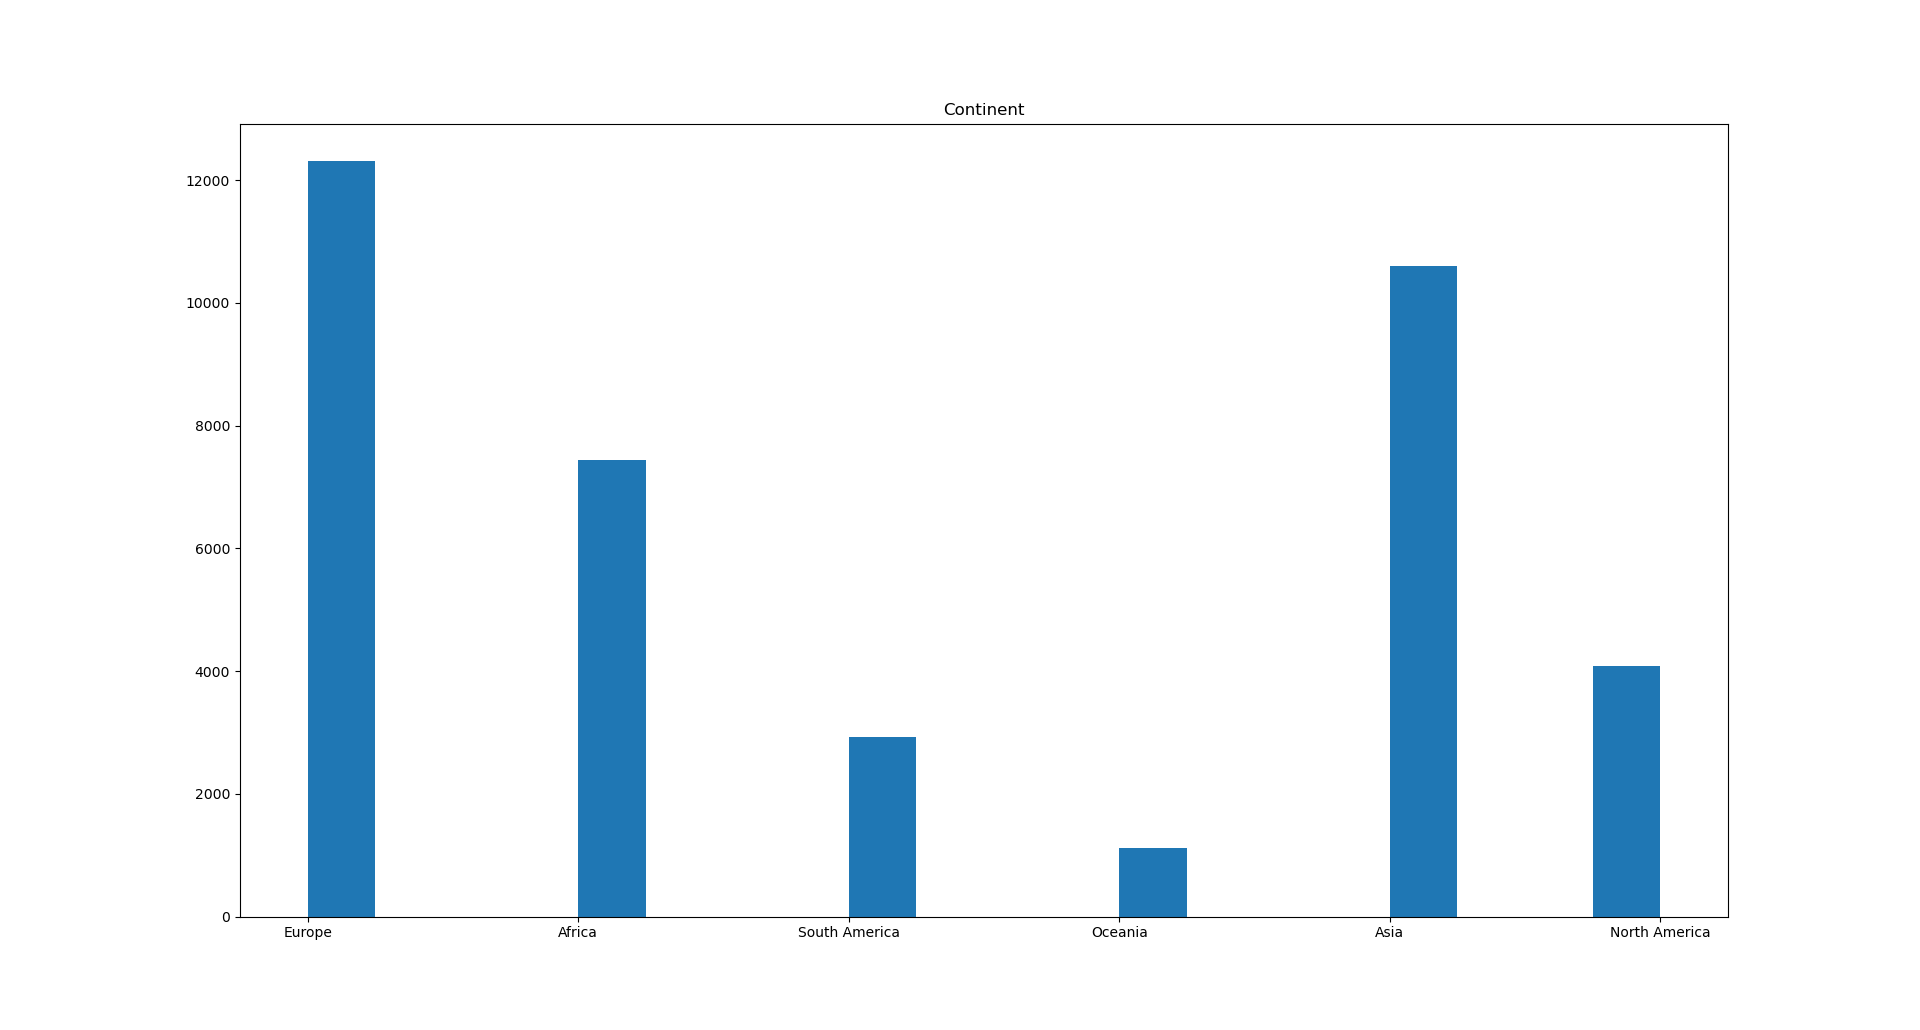
\includegraphics[width=\textwidth]{Figures/Question1/1. Histogram for Continent.png}
	\caption{Ιστόγραμμα για στήλη 'Continent'}
\end{figure}

\begin{figure}[H]
	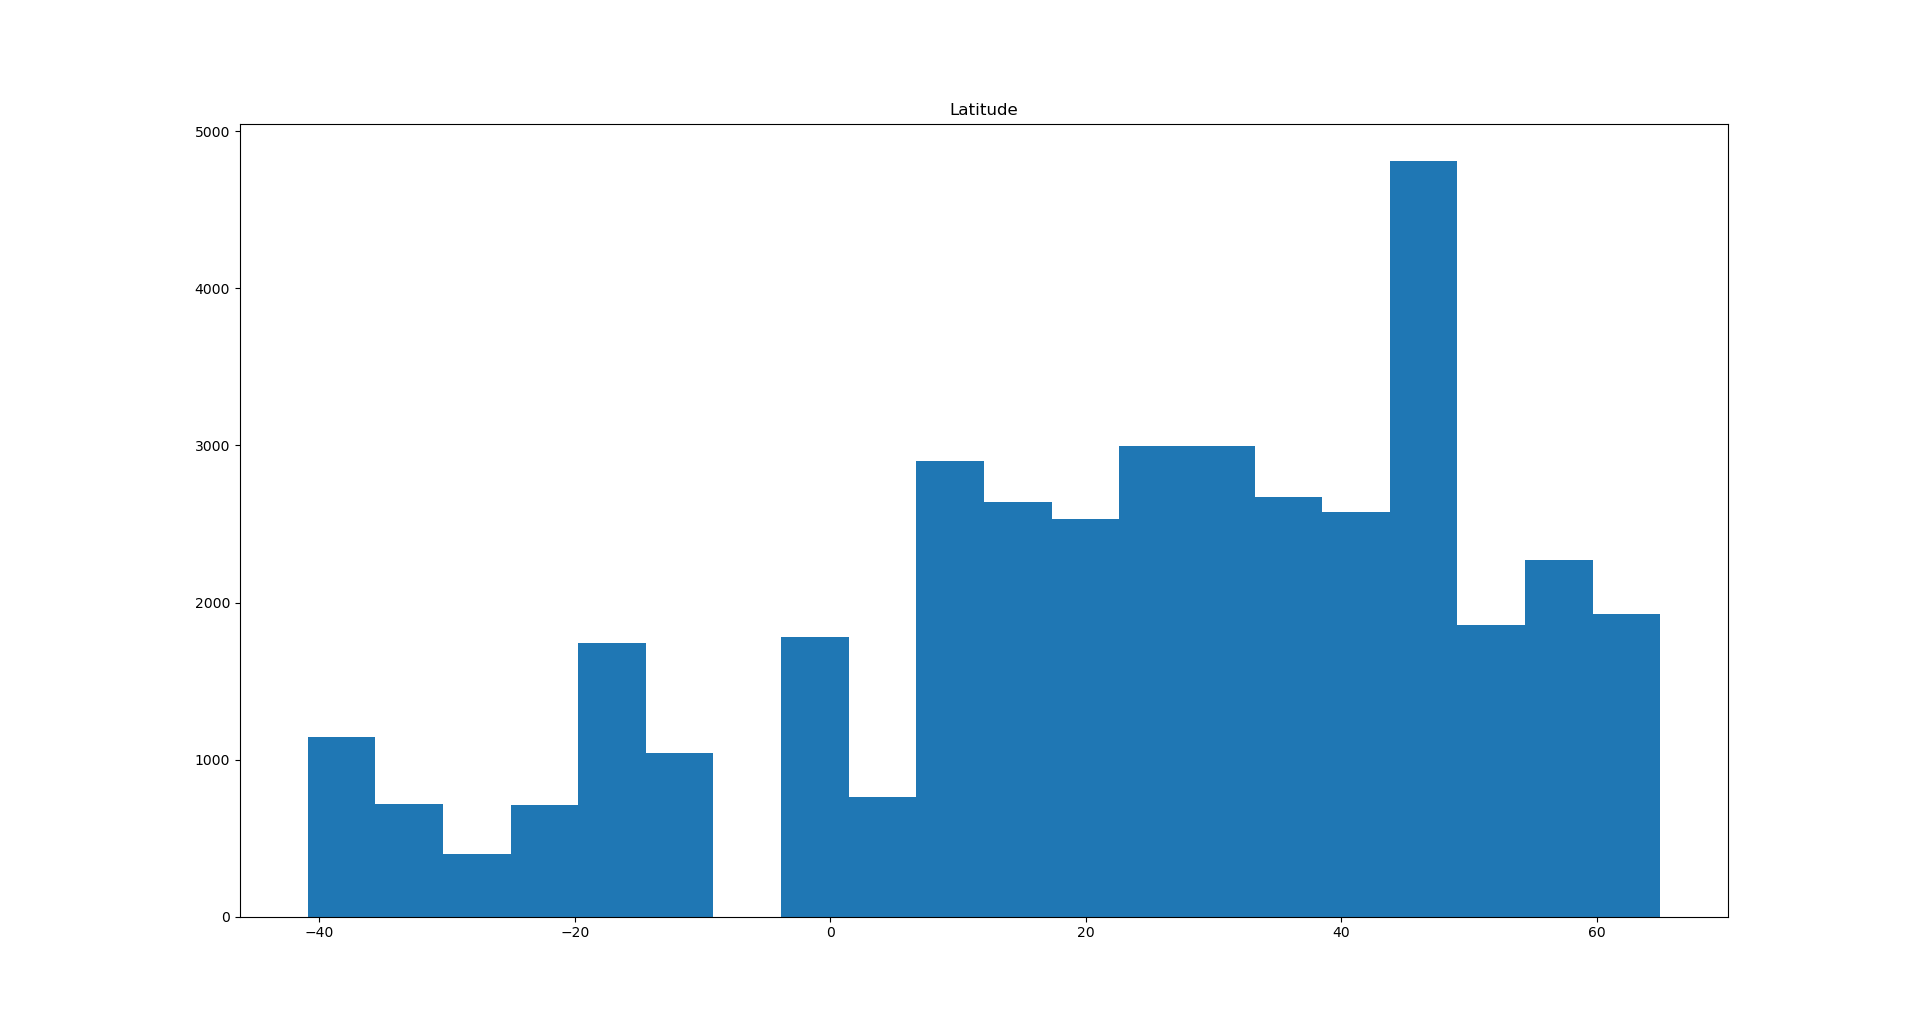
\includegraphics[width=\textwidth]{Figures/Question1/2. Histogram for Latitude.png}
	\caption{Ιστόγραμμα για στήλη 'Latitude'}
\end{figure}

\begin{figure}[H]
	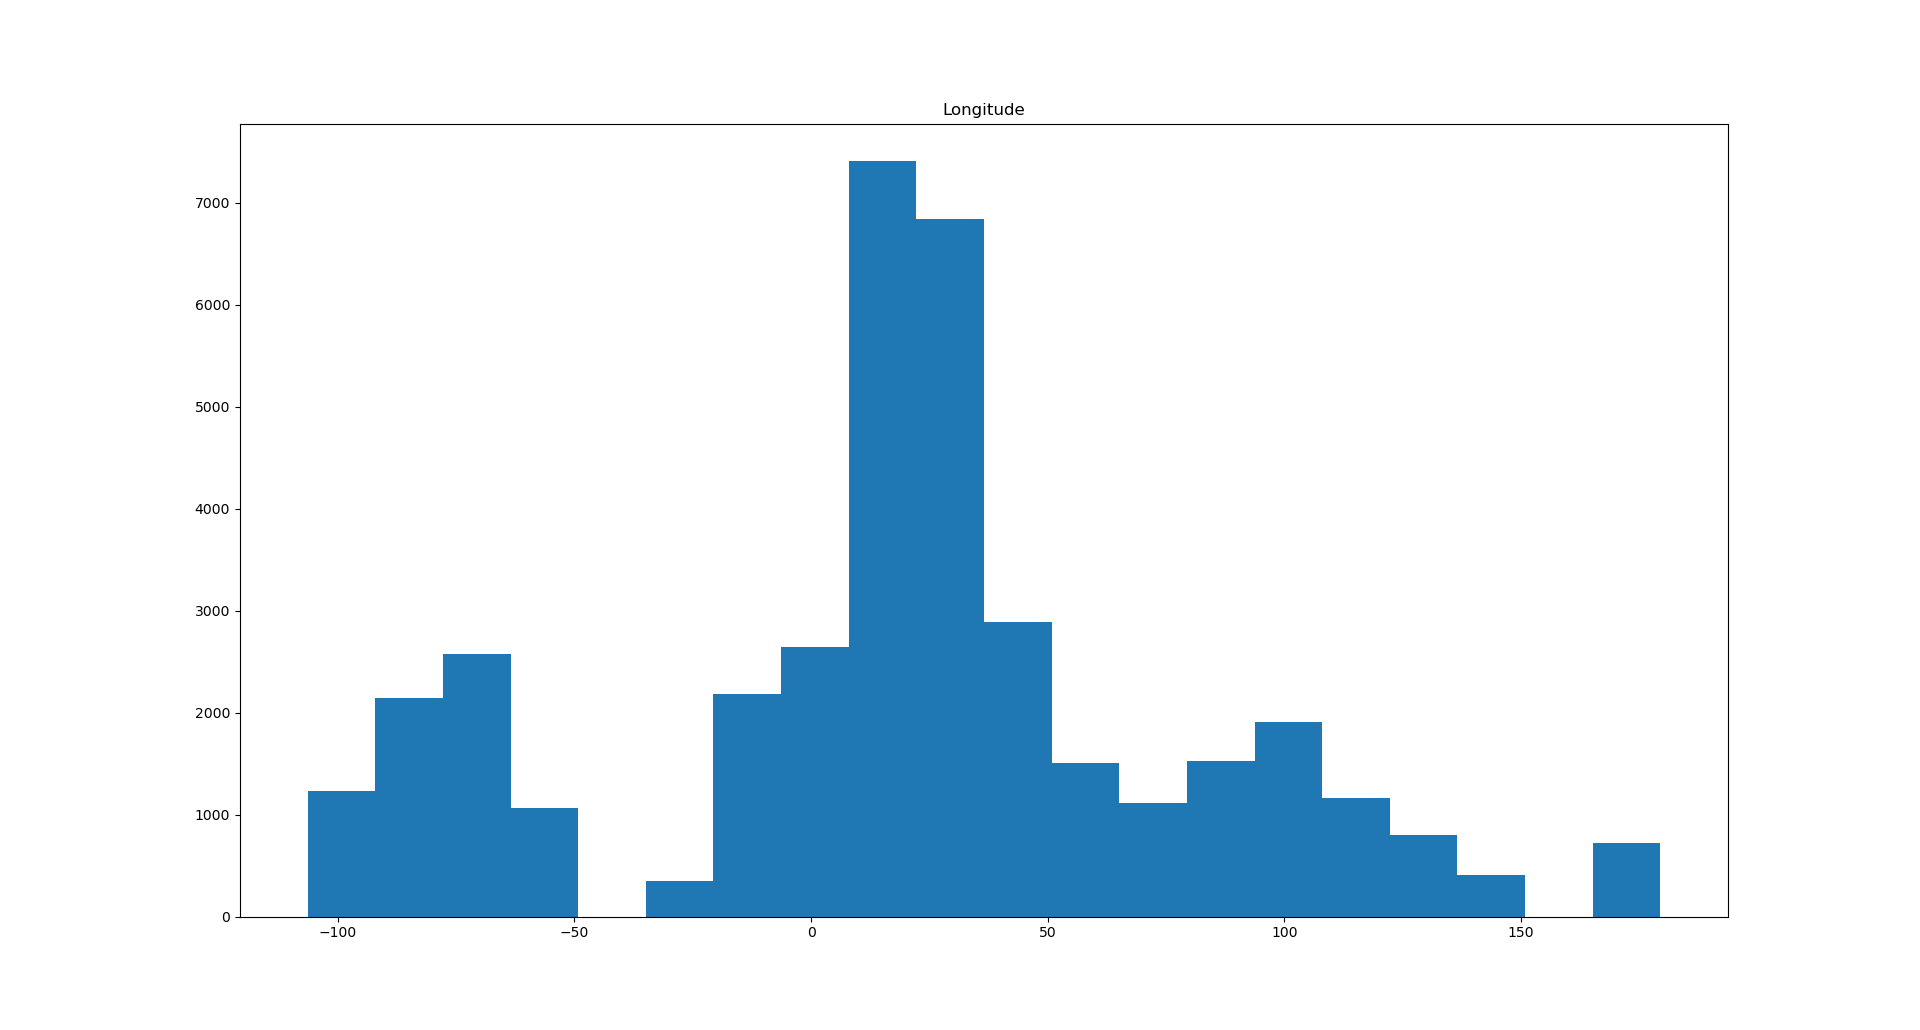
\includegraphics[width=\textwidth]{Figures/Question1/3. Histogram for Longtitude.png}
	\caption{Ιστόγραμμα για στήλη 'Longtitude'}
\end{figure}

\begin{figure}[H]
	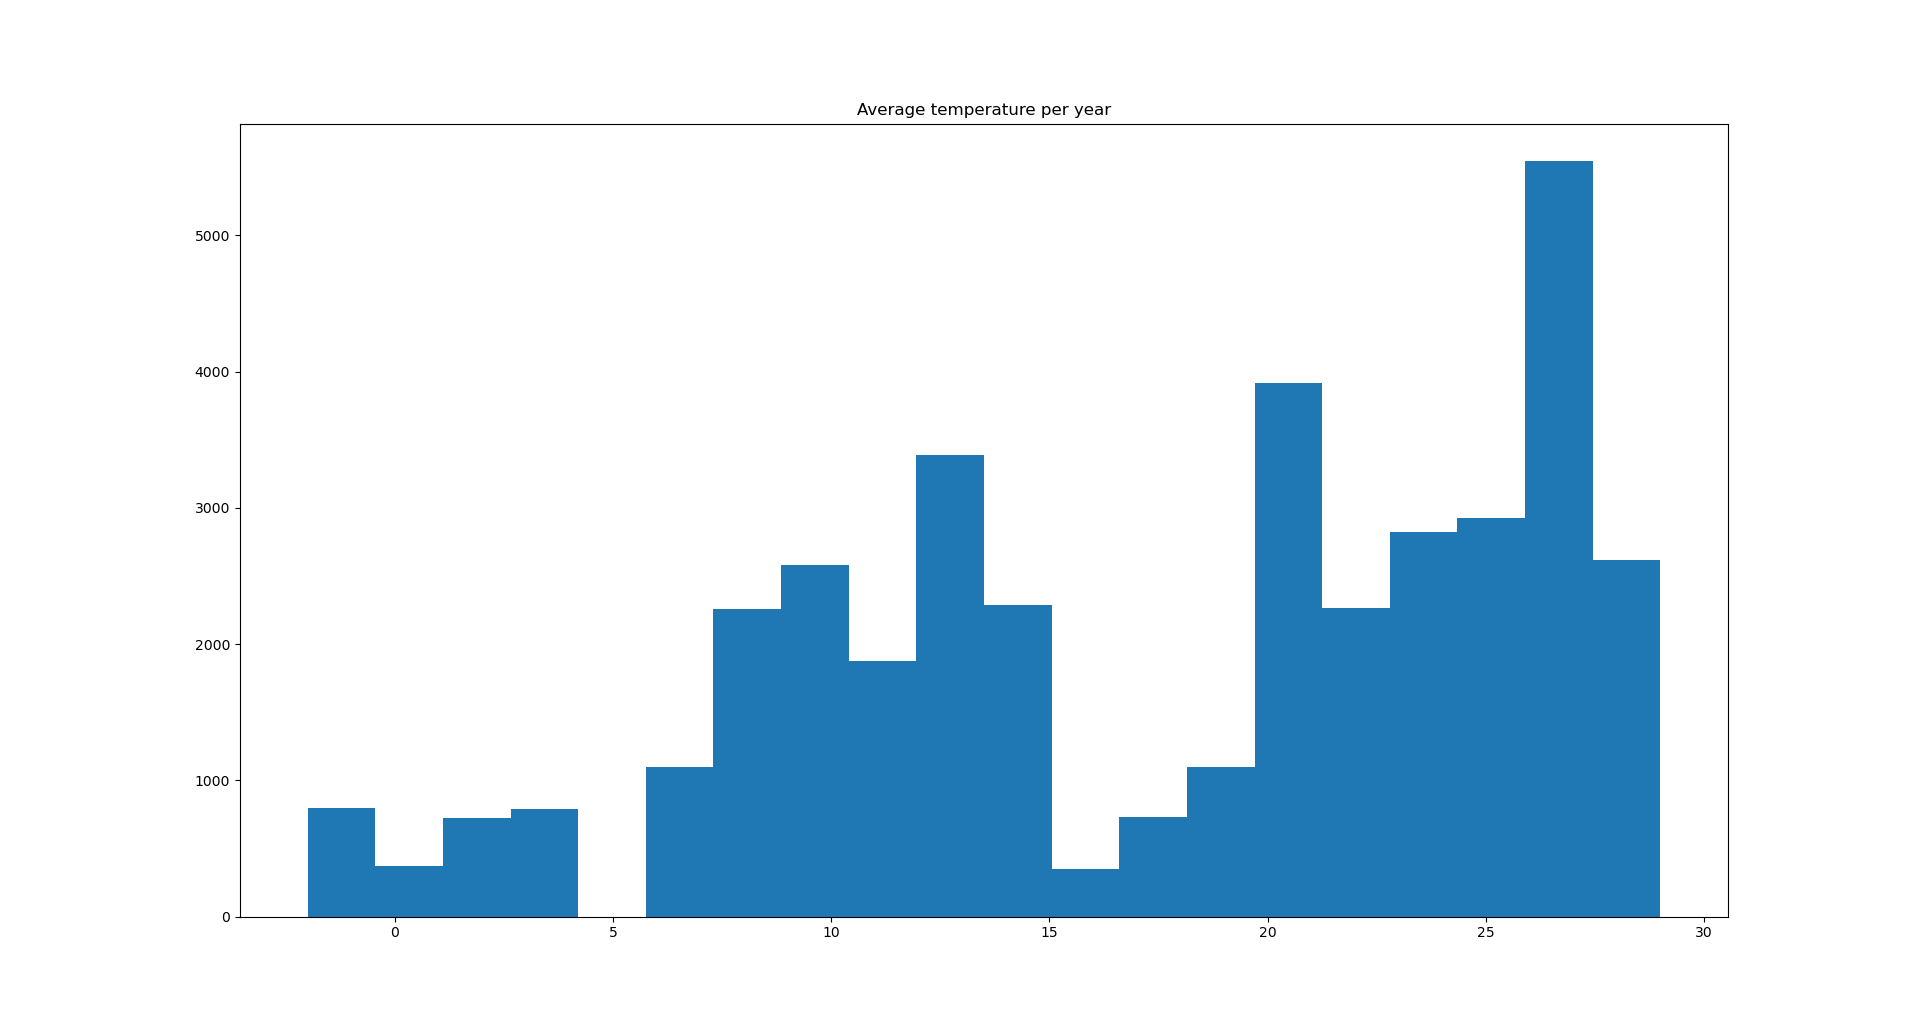
\includegraphics[width=\textwidth]{Figures/Question1/4. Histogram for average temperature per year.png}
	\caption{Ιστόγραμμα για στήλη 'Temperature'}
\end{figure}

\begin{figure}[H]
	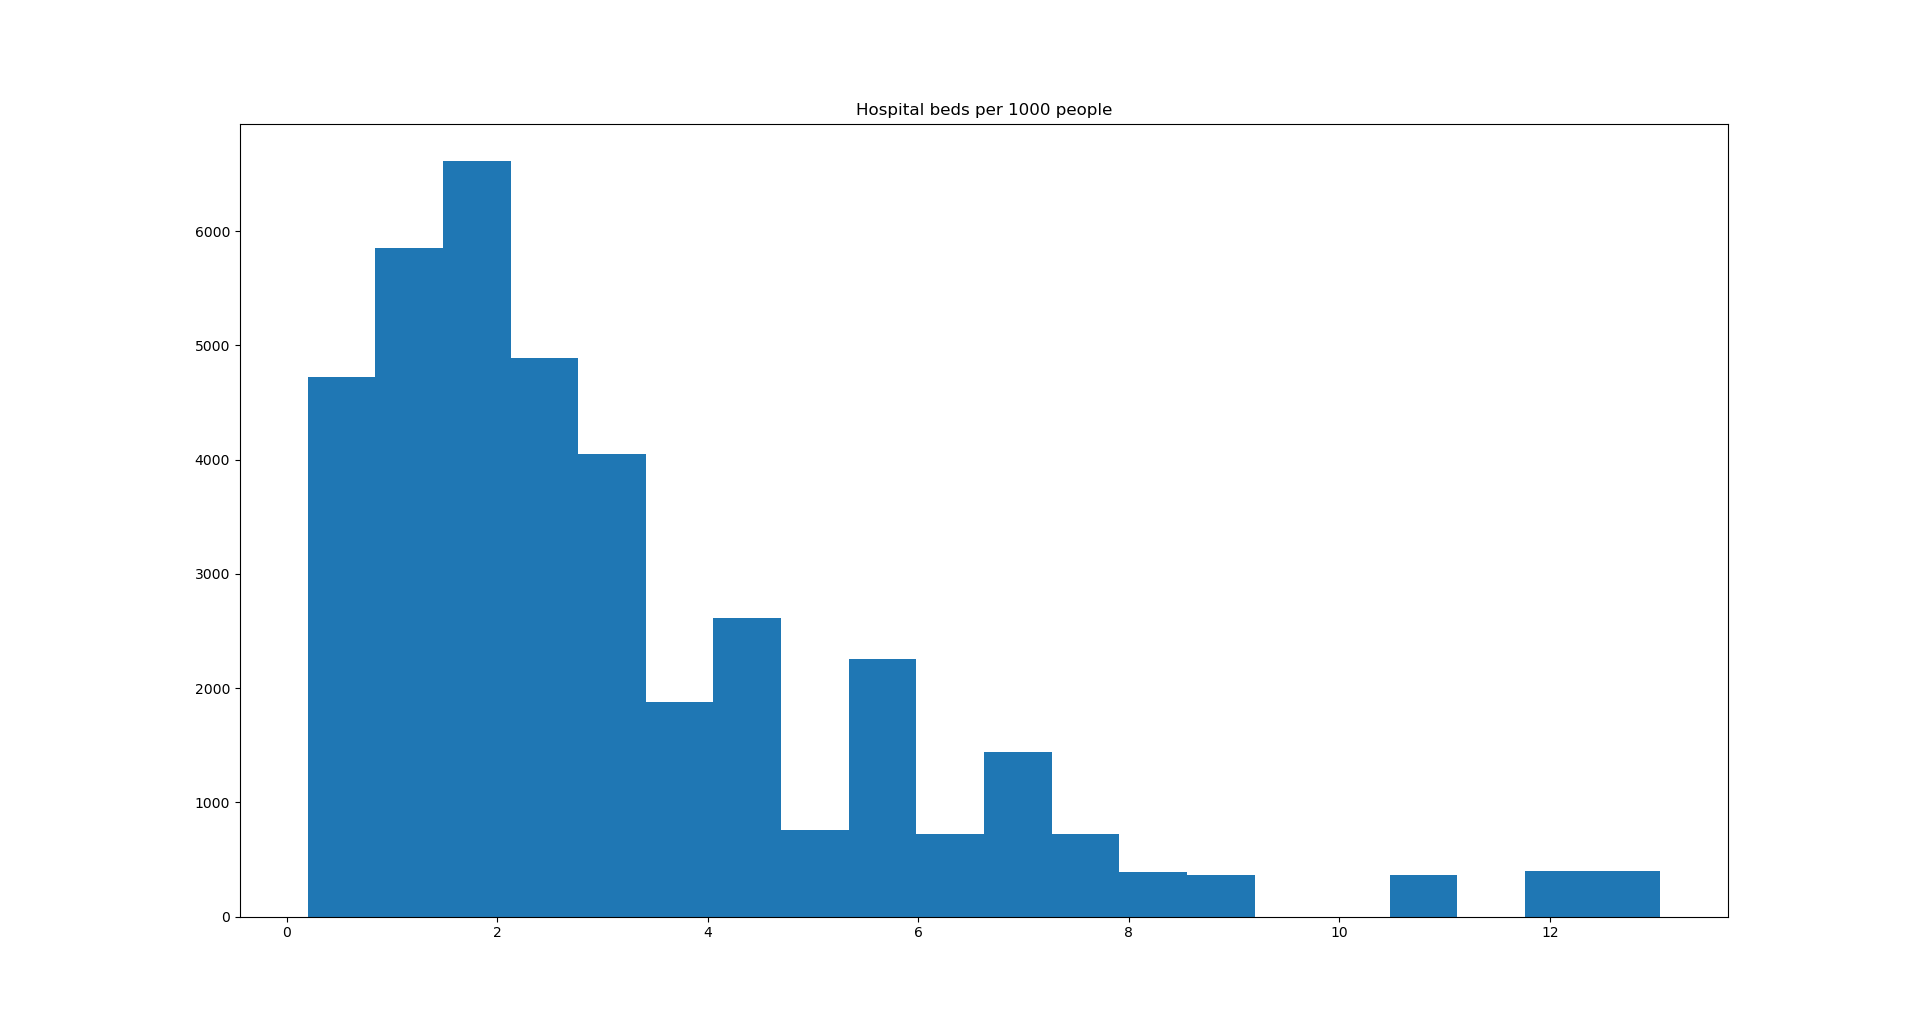
\includegraphics[width=\textwidth]{Figures/Question1/5. Histogram for hospital beds per 1000 people.png}
	\caption{Ιστόγραμμα για στήλη 'Hospital beds per 1000 people'}
\end{figure}

\begin{figure}[H]
	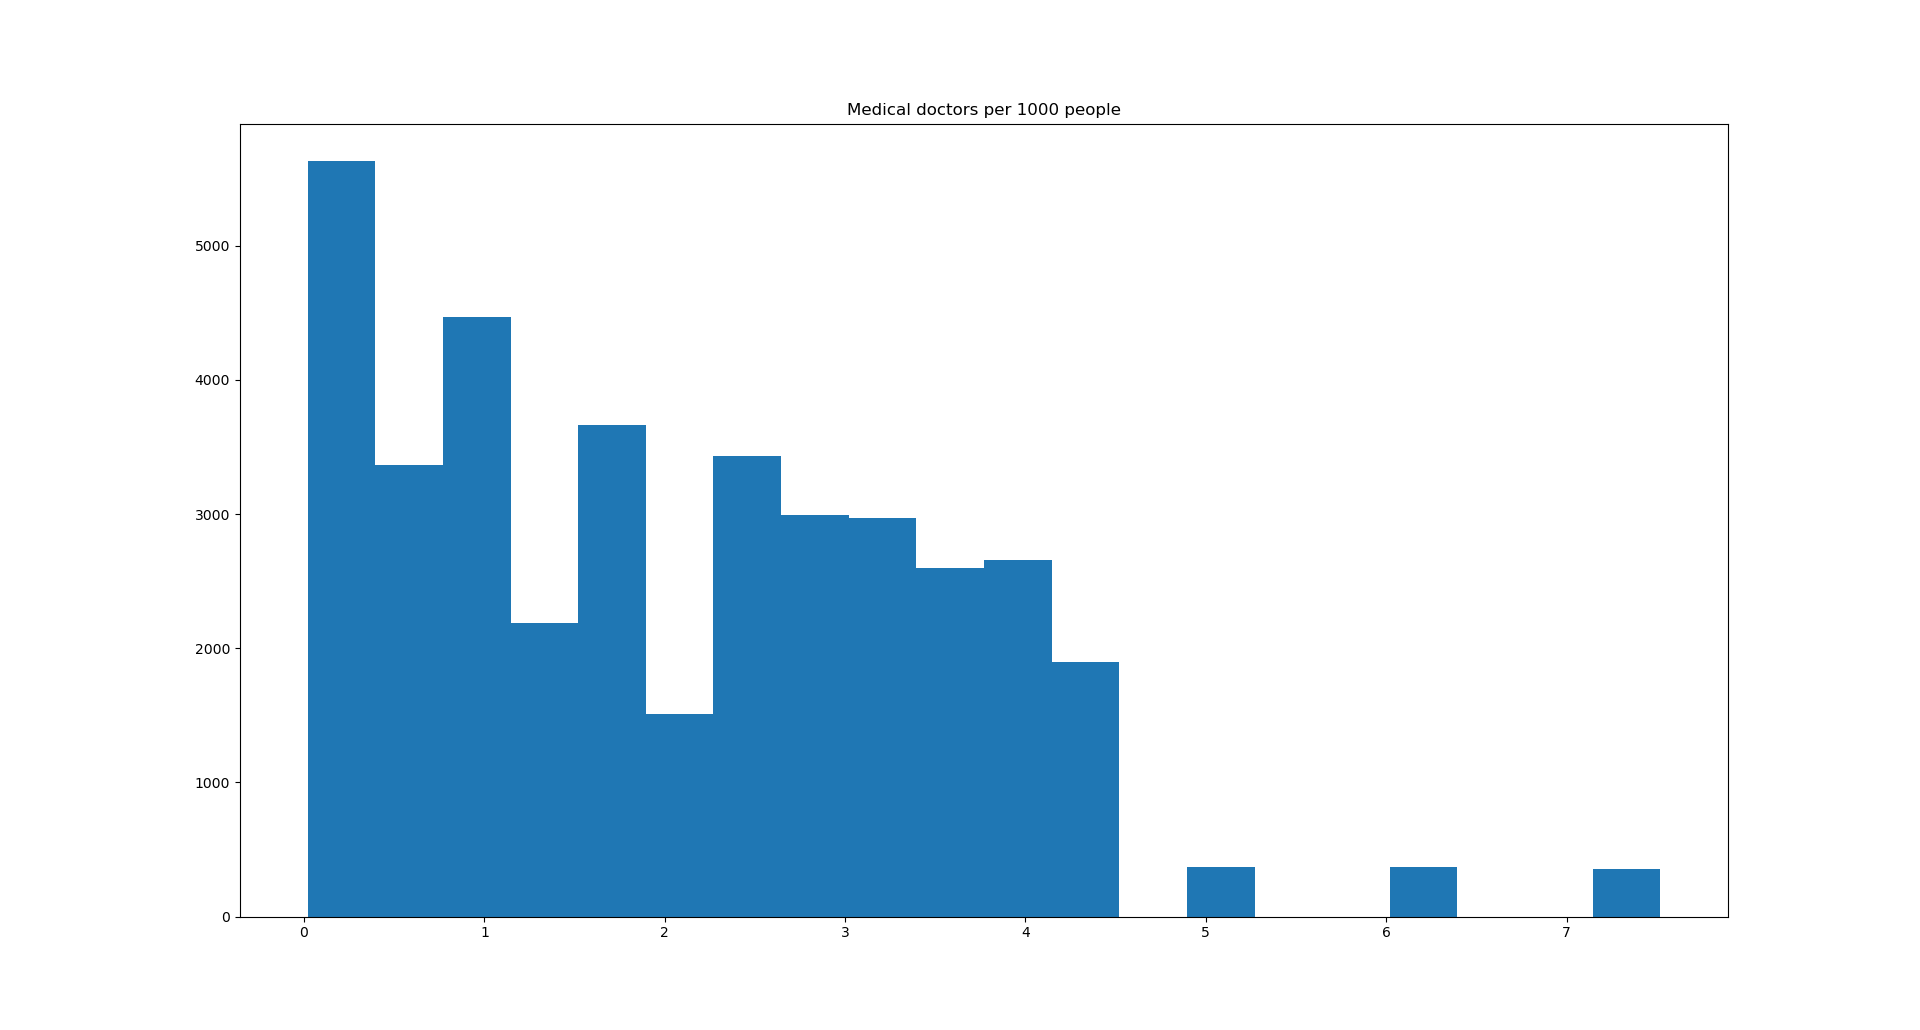
\includegraphics[width=\textwidth]{Figures/Question1/6. Histogram for medical doctors per 1000 people.png}
	\caption{Ιστόγραμμα για στήλη 'Medical doctors per 1000 people'}
\end{figure}

\begin{figure}[H]
	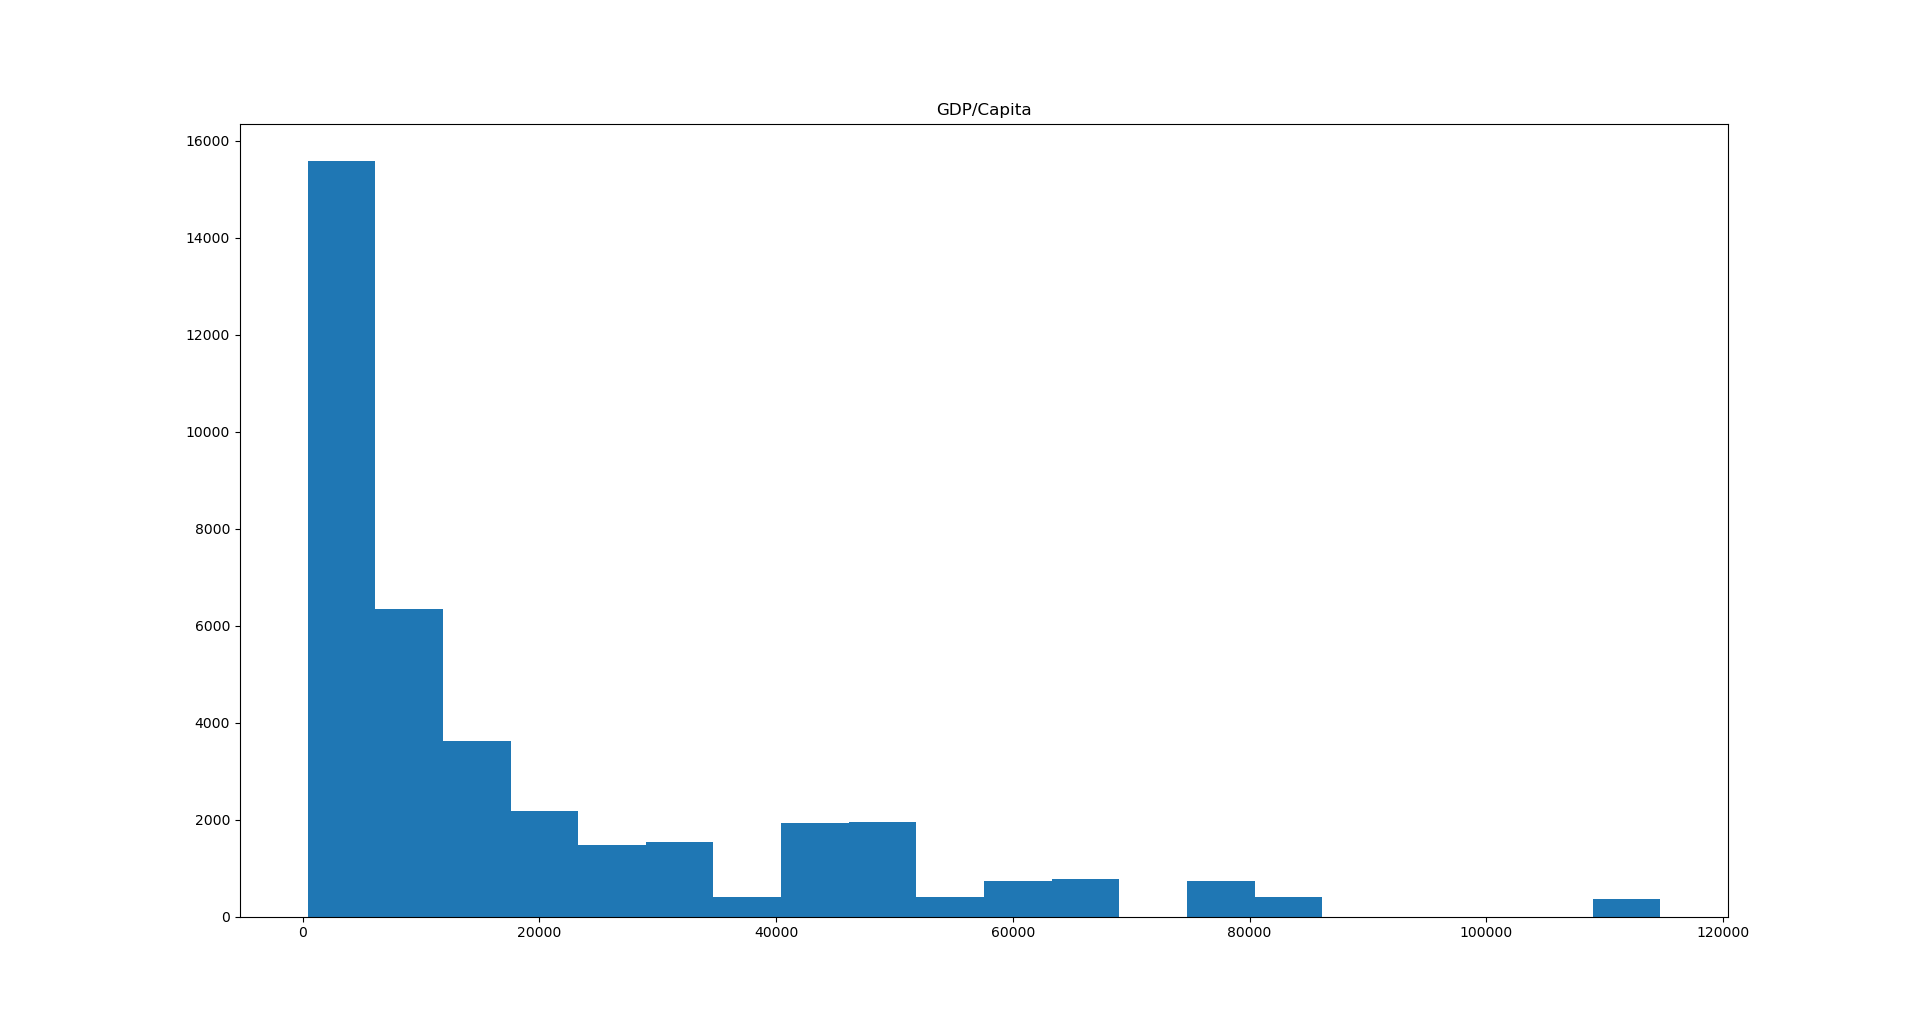
\includegraphics[width=\textwidth]{Figures/Question1/7. Histogram for GDP over capita.png}
	\caption{Ιστόγραμμα για στήλη 'GDP/Capita'}
\end{figure}

\begin{figure}[H]
	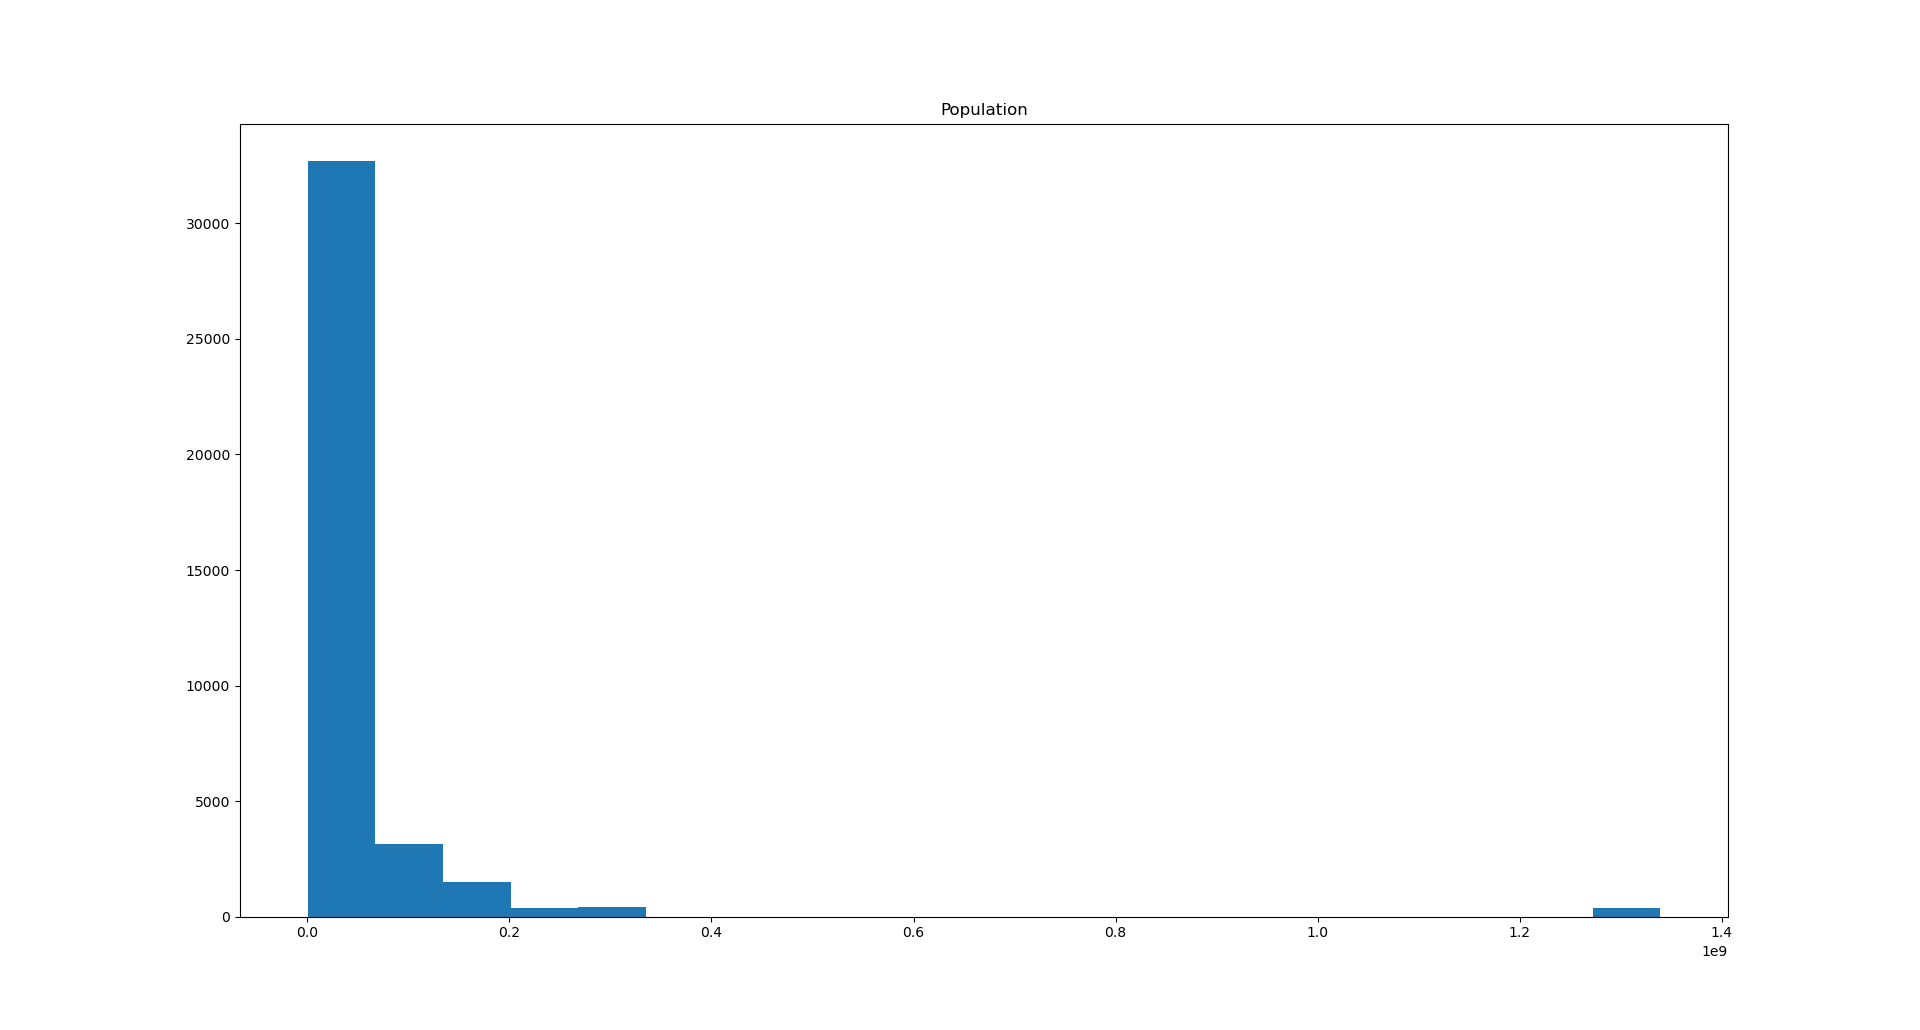
\includegraphics[width=\textwidth]{Figures/Question1/8. Histogram for population.png}
	\caption{Ιστόγραμμα για στήλη 'Population'}
\end{figure}

\begin{figure}[H]
	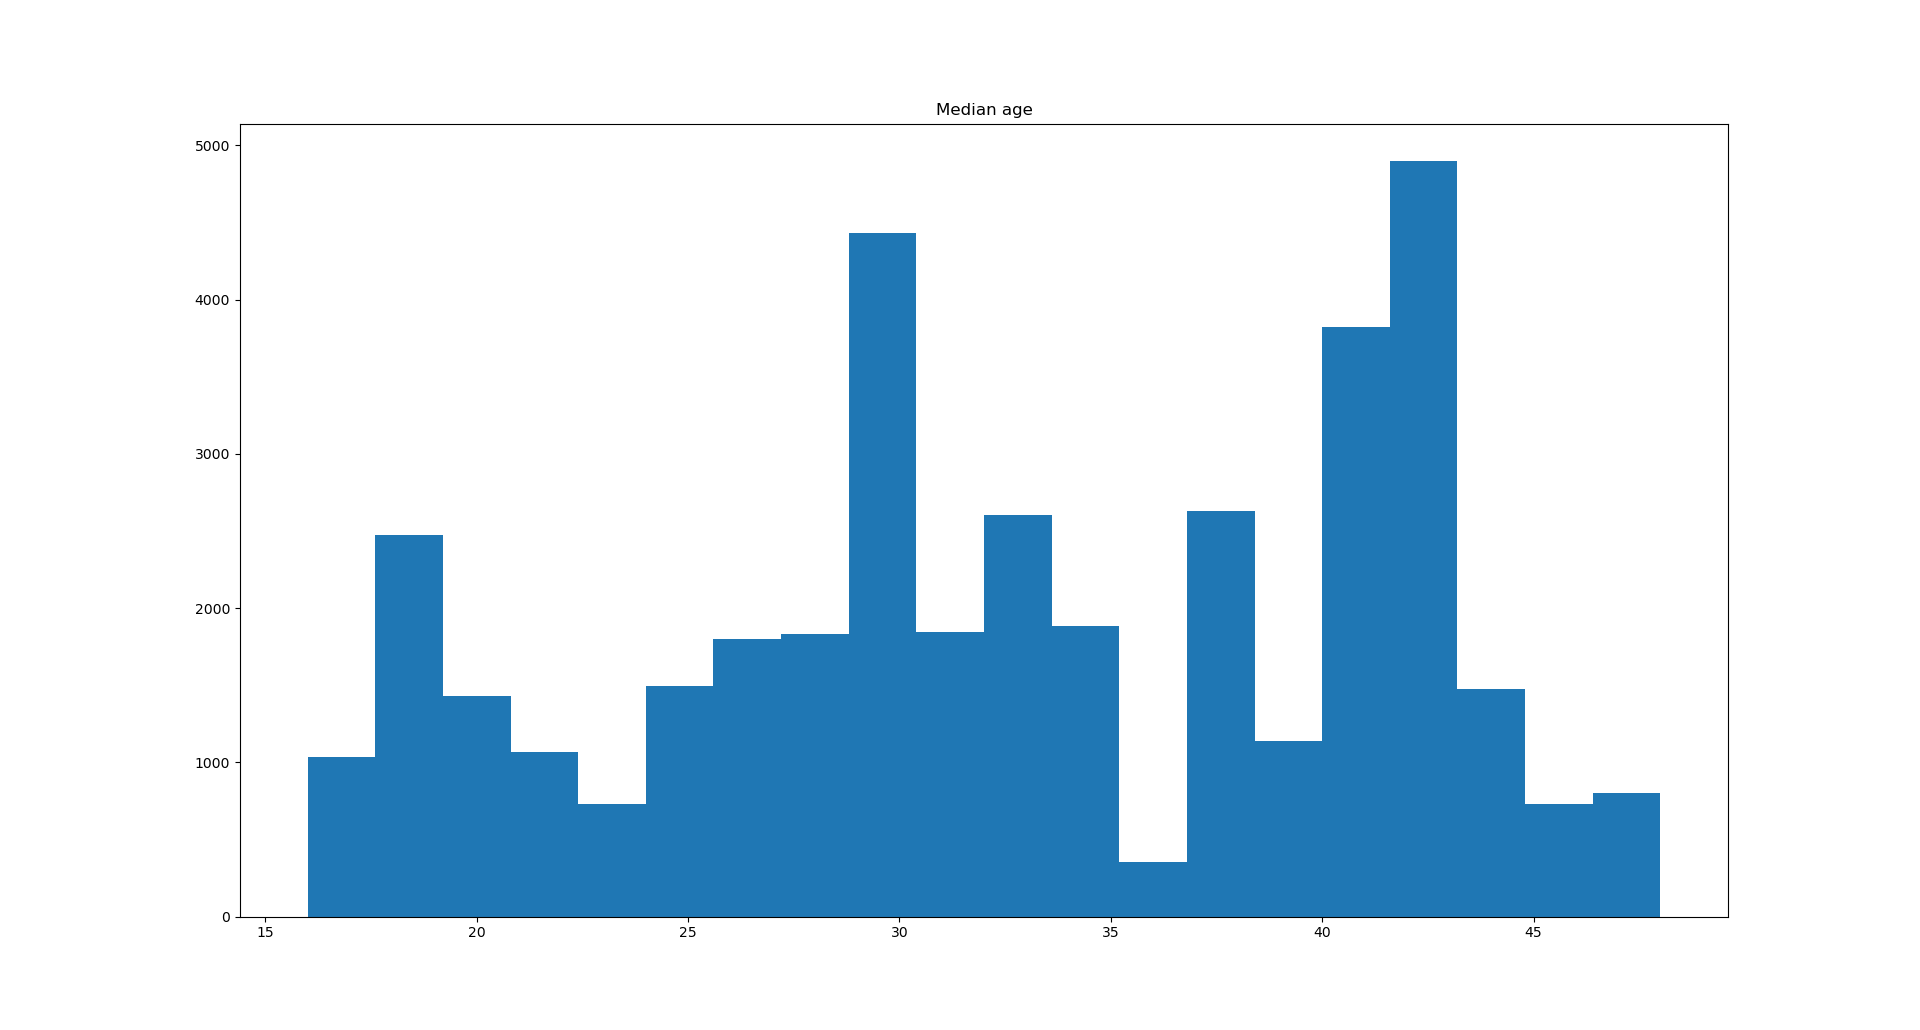
\includegraphics[width=\textwidth]{Figures/Question1/9. Histogram for median age.png}
	\caption{Ιστόγραμμα για στήλη 'Median age'}
\end{figure}

\begin{figure}[H]
	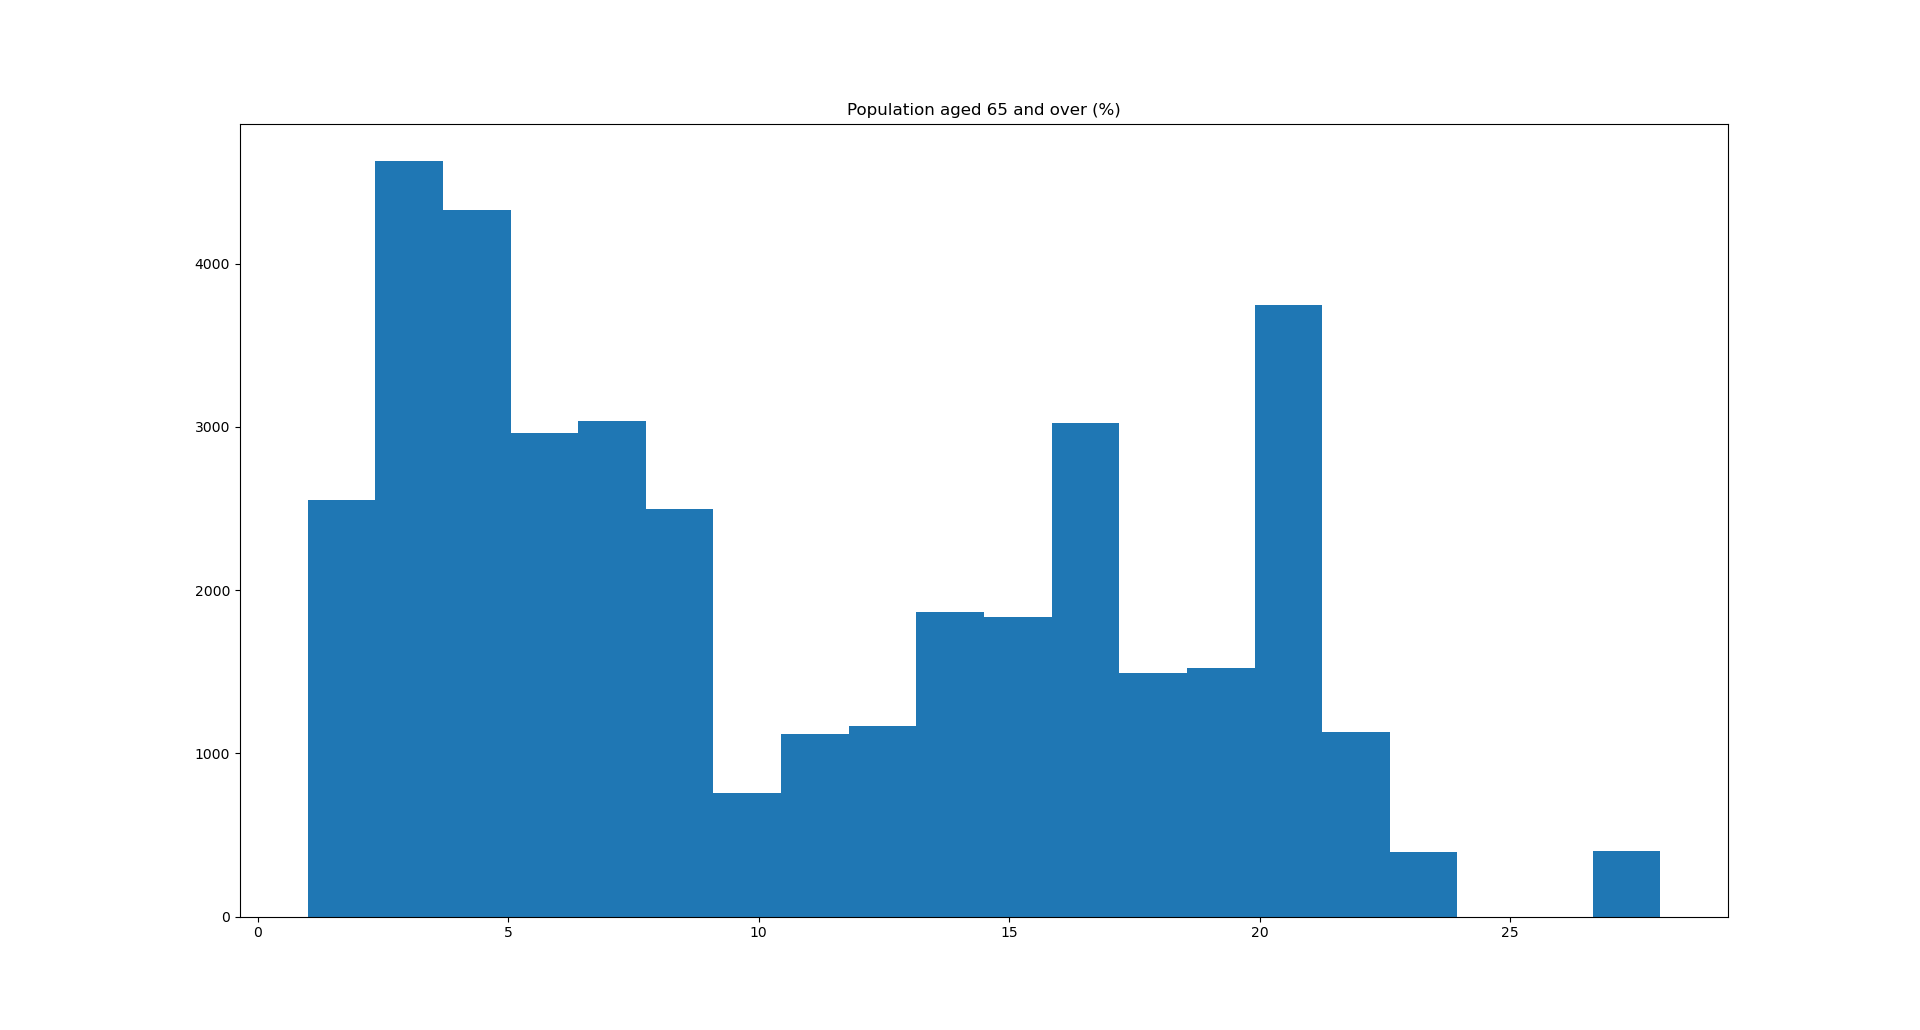
\includegraphics[width=\textwidth]{Figures/Question1/10. Histogram for population aged 65 and over.png}
	\caption{Ιστόγραμμα για στήλη 'Population aged 65 and over (\%)'}
\end{figure}

\begin{figure}[H]
	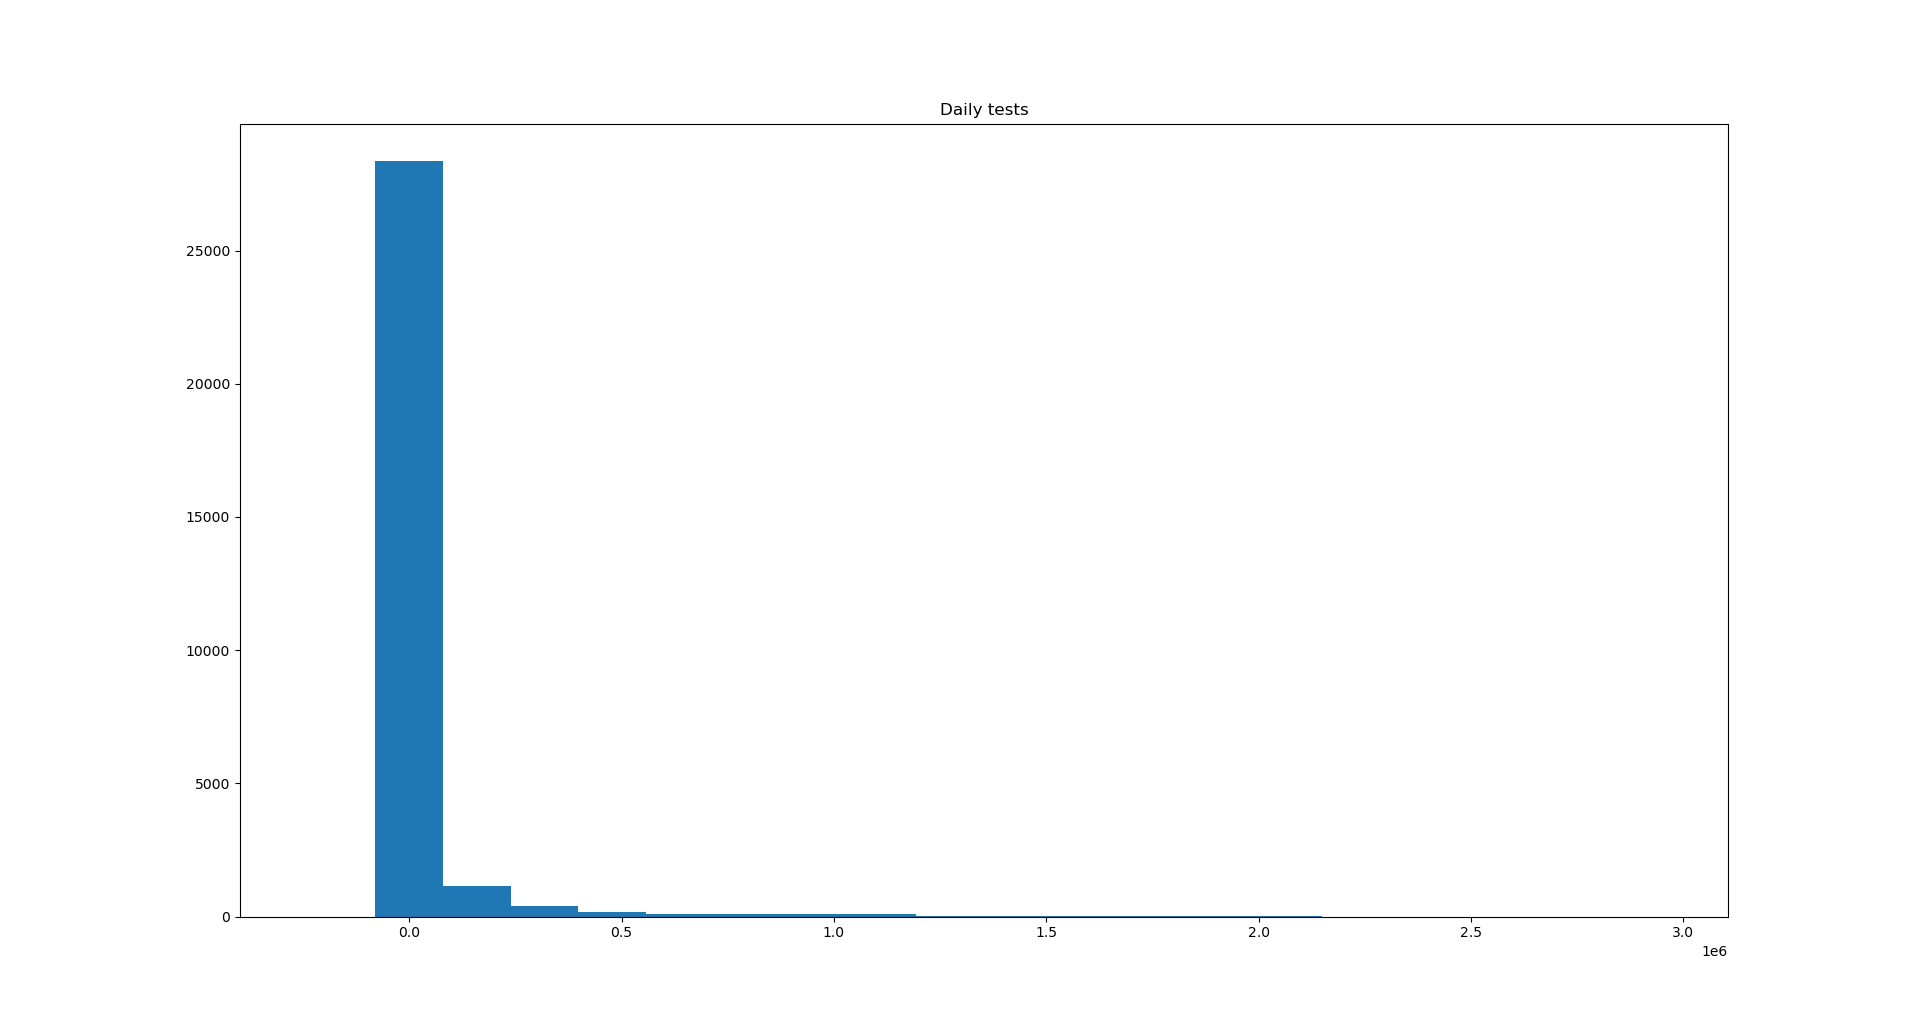
\includegraphics[width=\textwidth]{Figures/Question1/11. Histogram for daily tests.png}
	\caption{Ιστόγραμμα για στήλη 'Daily tests'}
\end{figure}

\begin{figure}[H]
	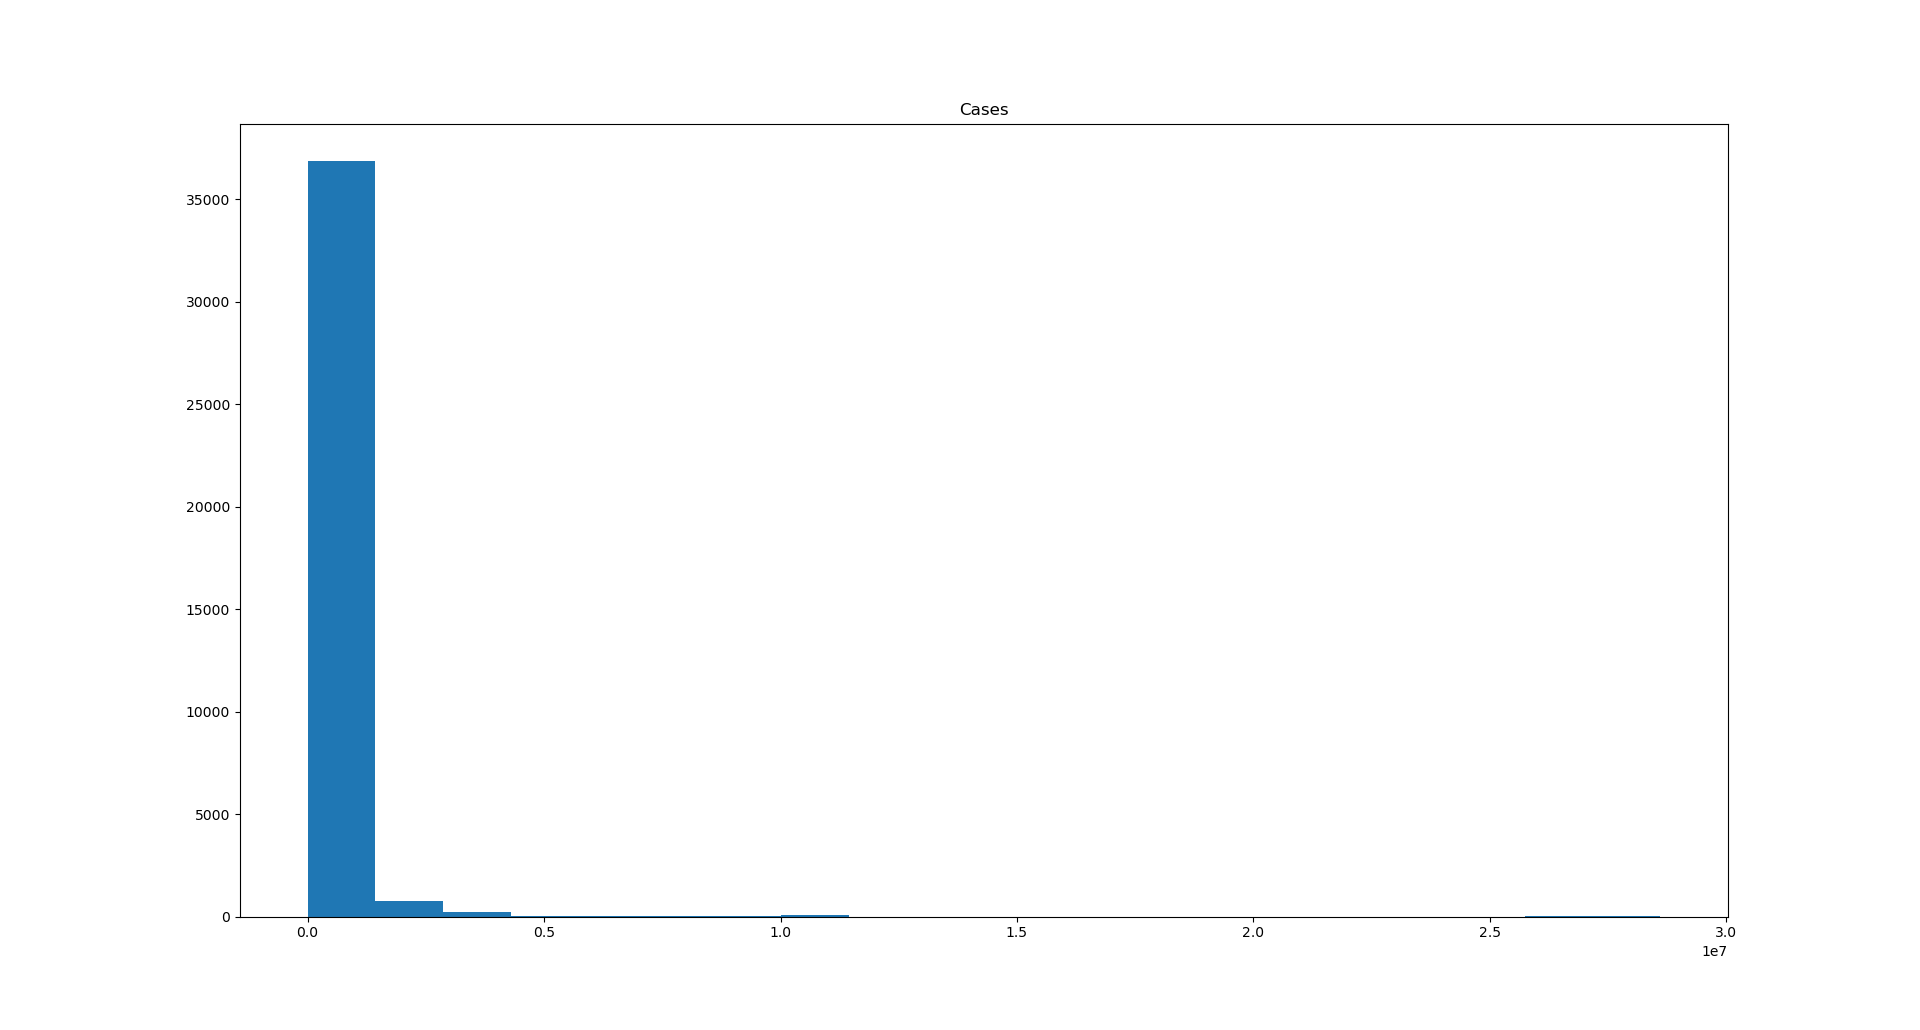
\includegraphics[width=\textwidth]{Figures/Question1/12. Histogram for cases.png}
	\caption{Ιστόγραμμα για στήλη 'Cases'}
\end{figure}

\begin{figure}[H]
	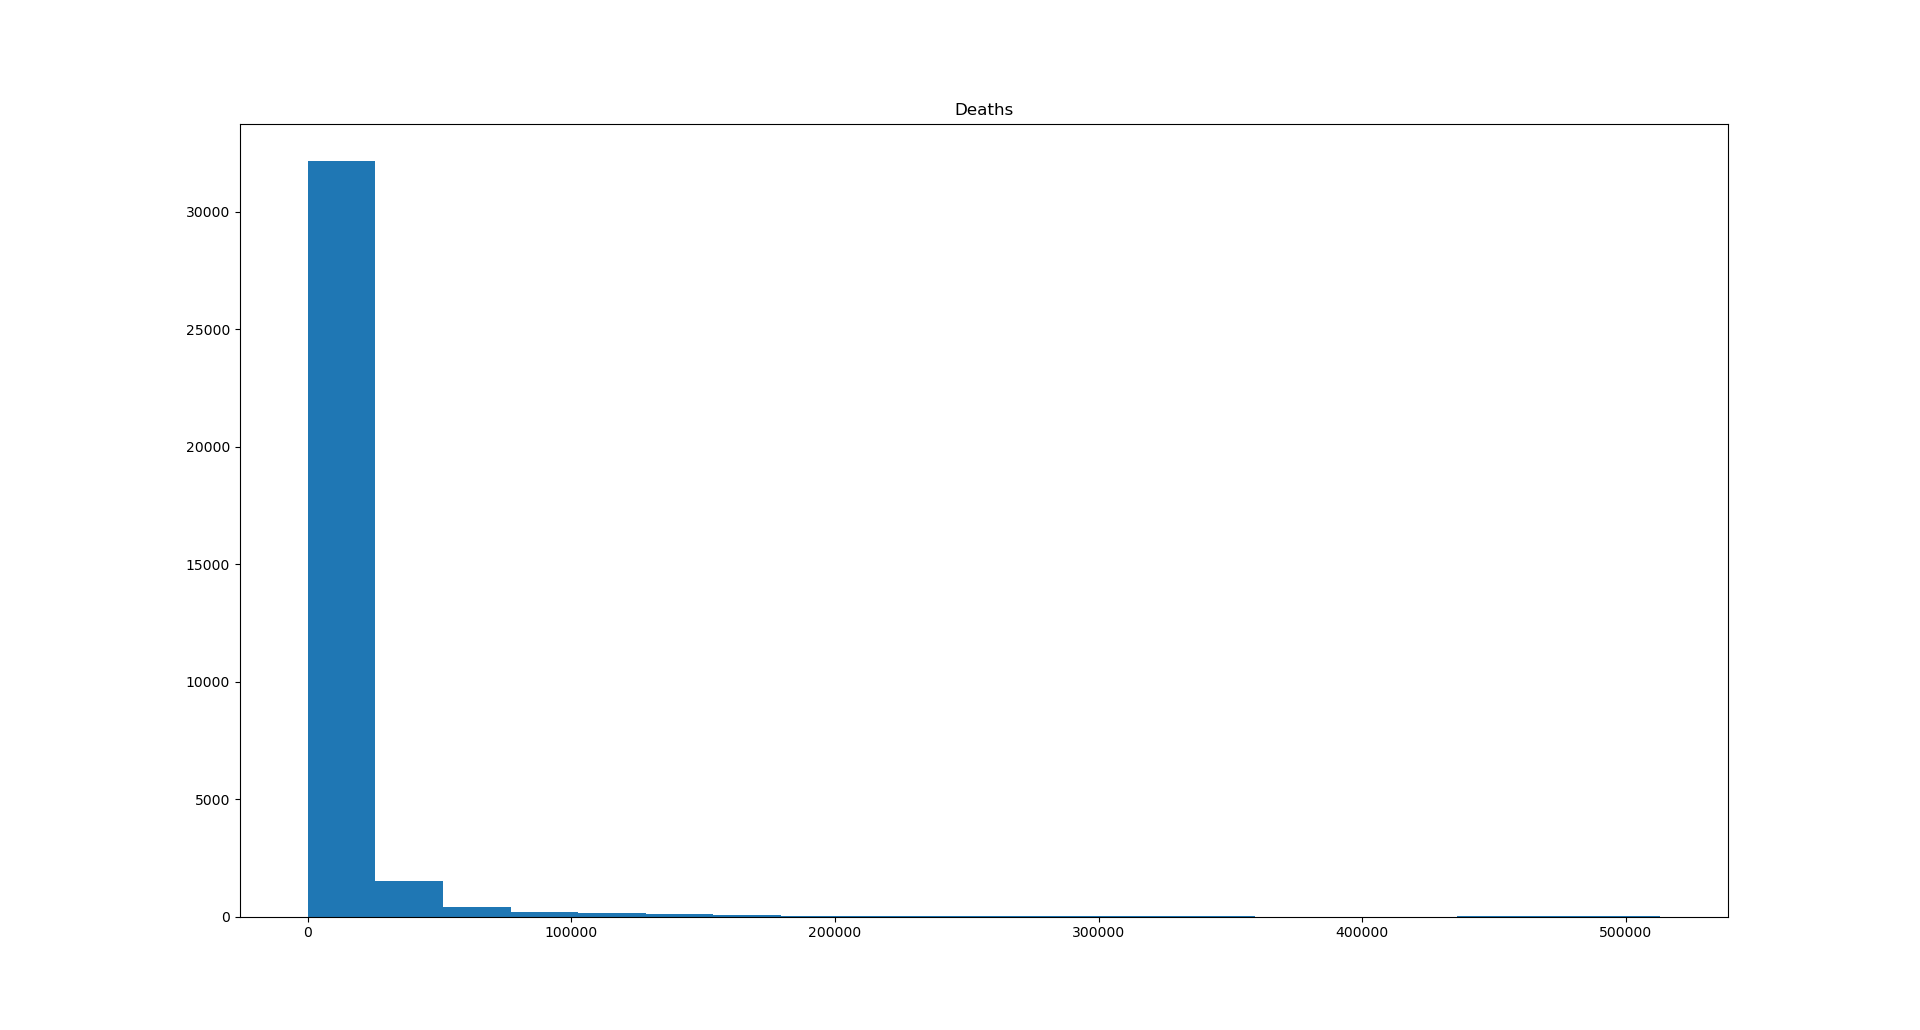
\includegraphics[width=\textwidth]{Figures/Question1/13. Histogram for deaths.png}
	\caption{Ιστόγραμμα για στήλη 'Deaths'}
\end{figure}

Τέλος παρακάτω παρουσιάζουμε το Correlation Matrix Heatmap που φτιάξαμε για τις στήλες του dataset.

\begin{figure}[H]
	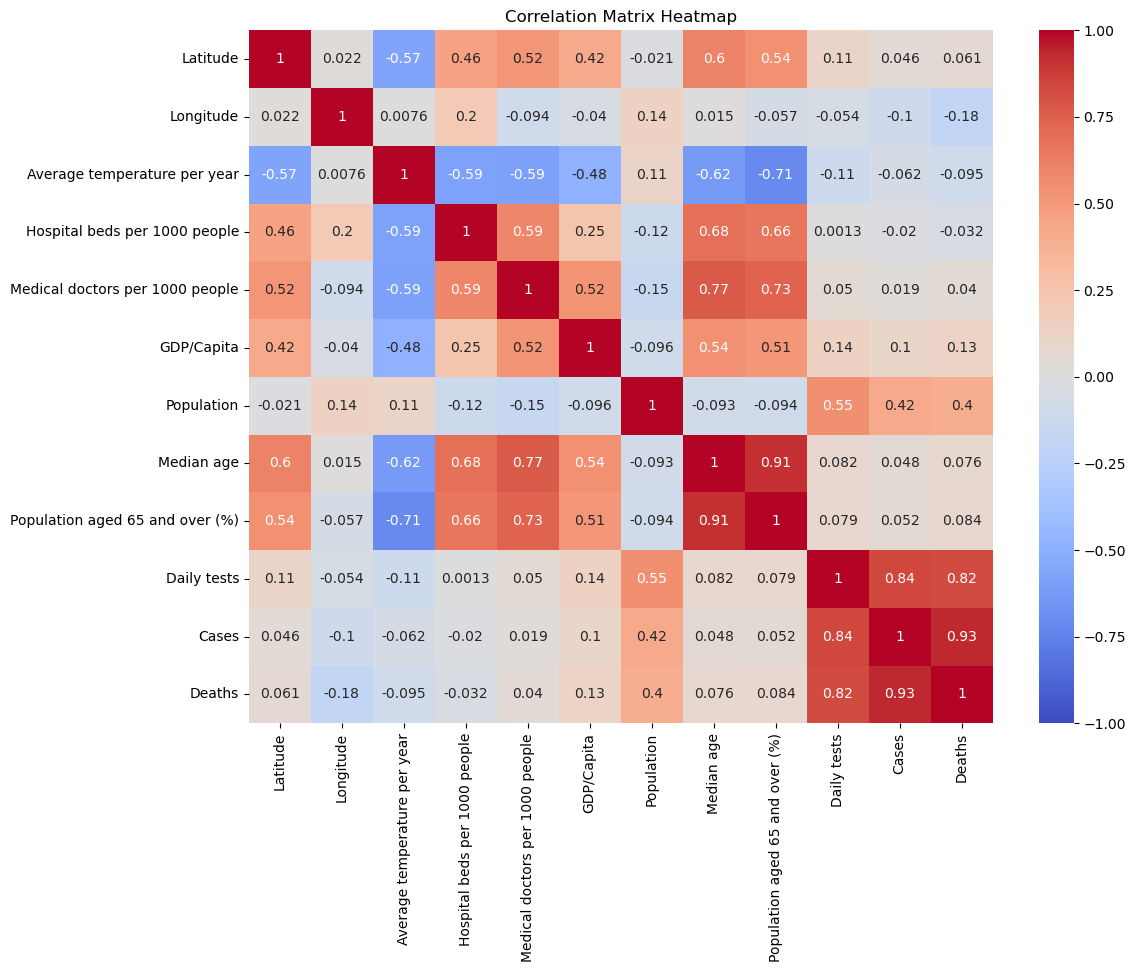
\includegraphics[width=\textwidth]{Figures/Question1/14. Correlation matrix heatmap.png}
	\caption{Correlation Matrix Heatmap για τις στήλες}
\end{figure}

\subsubsection{Συμπεράσματα}

Από τα στατιστικά στοιχεία και τα ιστογράμματα συμπεραίνουμε πως πολλές από τις στήλες περιέχουν στοιχεία που φαίνεται να αποτελούν half-normal κατανομές, με διαφορετικές τιμές μέσης τιμής και διασποράς. Οι στήλες αυτές είναι οι 'Medical doctors per 1000 people', 'GDP/Capita', 'Population', 'Daily tests', 'Cases', 'Deaths'. Επίσης η στήλη 'Hospital beds per 1000 people' φαίνεται να ακολουθεί log-normal κατανομή. Για τις υπόλοιπες στήλες δεν μπορούμε να συμπεράνουμε ότι ανήκουν σε κάποια κατανομή.

Από το Correlation Matrix Heatmap παρατηρούμε ότι υπάρχει μεγάλη συσχέτιση μεταξύ 'Daily tests', 'Cases' και 'Deaths', καθώς και μεταξύ 'Median age', 'People aged 65 and over (\%)', 'Hospital beds per 1000 people' και 'Medical doctors per 1000 people'. Υπάρχει επίσης μεγάλη αρνητική συσχέτιση μεταξύ του 'Average Temperature per year' σε σχέση με τα 'Population aged 65 and over (\%)', 'Median age', 'Medical doctors per 1000 people', 'Hospital beds per 1000 people' και 'Latitude'. Σημειώνουμε ότι υπάρχουν και άλλες συσχετίσεις εκτός από αυτές που αναφέρονται, αλλά δεν είναι τόσο ισχυρές όσο αυτές που αναφέρουμε εδώ, οπότε τις παραλείπουμε για λόγους συντομίας, εφόσον φαίνονται και στο heatmap.

\section{Υλοποίηση και Αποτελέσματα Ερωτήματος 2}

\subsection{Σύντομη Περιγραφή της Διαδικασίας Υλοποίησης}

\subsubsection{Χειρισμός Τιμών που Λείπουν}

Για την υλοποίηση του ερωτήματος αυτού, αρχικά αφού διαβάσουμε το αρχείο του dataset θα πρέπει να αντιμετωπίσουμε τις τιμές που λείπουν από αυτό. Αυτό το επιτυγχάνουμε με τη χρήση των εντολών:

\begin{lstlisting}[language=Python]
df = df.groupby('Entity',group_keys=False).apply(lambda x: x.fillna(method='ffill'))
df = df.groupby('Entity',group_keys=False).apply(lambda x: x.fillna(method='bfill'))
\end{lstlisting}

Αυτές οι εντολές επιτυγχάνουν αρχικά το grouping του DataFrame με βάση το 'Entity' (χώρα) και μετά την εφαρμογή της fillna μεθόδου, η οποία συμπληρώνει τις τιμές που λείπουν αρχικά με χρήση forward fill στη πρώτη εντολή και έπειτα με backward fill στη δεύτερη εντολή.

Το forward fill επιτυγχάνει την αντικατάσταση τιμών που λείπουν με την τελευταία προηγούμενη καταγεγραμμένη τιμή, αλλά επειδή γίνεται να υπάρχουν ακόμα κενά (πχ αν λείπουν τιμές στην αρχή των καταγεγραμμένων στοιχείων), κάνουμε έπειτα το backward fill που συμπληρώνει τιμές που λείπουν με την επόμενη καταγεγραμμένη τιμή.

Ο λόγος που προτιμούμε πρώτα να κάνουμε forward fill και μετά backward fill είναι επειδή με αυτόν τον τρόπο ελαχιστοποιούμε την συμπλήρωση με βάση τις μελλοντικές ως προς τη χρονική στιγμή που συμπληρώνουμε τιμές.

Έπειτα αφαιρούμε όλα τα duplicates που τυχόν προέκυψαν με χρήση της μεθόδου drop\_duplicates() του Pandas.

\subsubsection{Δημιουργία Νέων Πεδίων για το Clustering}

Αποφασίσαμε για το πιο αποτελεσματικό clustering να προσθέσουμε ορισμένα πεδία στα δεδομένα τα οποία εξάγονται από τα υπόλοιπα δεδομένα. Πιο συγκεκριμένα τα νέα πεδία αυτά τα ορίζουμε ως εξής:

\begin{itemize}
    \item Positive Ratio = Today's New Cases / Daily Tests
    \item Death Ratio = Today's Deaths / New Cases
    \item Tested Ratio = Daily Tests / Population
\end{itemize}

\subsubsection{Προεπεξεργασία Δεδομένων}

Το πρώτο βήμα της προεπεξεργασίας θα είναι να κάνουμε aggregation των δεδομένων. Έτσι αντί να αποθηκεύουμε για κάθε χώρα τα δεδομένα κάθε μέρας ξεχωριστά, θα αποθηκεύσουμε είτε τον μέσο όρο είτε την τελευταία τιμή μιας στήλης δεδομένων κάθε φορά. Αυτό μας διευκολύνει στο clustering, επειδή μειώνει τον όγκο των δεδομένων εισόδου και ταυτόχρονα απομονώνει την σημαντική πληροφορία από τα δεδομένα για όλες τις ημέρες. Έτσι θα αποθηκεύσουμε τη μέση τιμή των 'Positive Ratio', 'Death Ratio', και 'Tested Ratio' και θα αποθηκεύσουμε και την τελευταία τιμή που εμφανίζεται για όλα τα υπόλοιπα Series.

Επειδή το 'Continent' περιέχει κατηγορικά δεδομένα, αποφασίζουμε να τα μετατρέψουμε σε αριθμητικά δεδομένα ώστε να μπορέσουμε να κάνουμε κανονικοποίηση αργότερα πάνω σε αυτά. Άρα κάνουμε one-hot encoding για όλο το Series 'Continent' πάνω στο DataFrame που προέκυψε από το προηγούμενο βήμα.

Έπειτα αφαιρούμε το Series 'Date' από το DataFrame των προηγούμενων βημάτων, επειδή αυτό είναι ίδιο σε κάθε περίπτωση (ίσο με την τελευταία ημερομηνία του dataset).

Τέλος κάνουμε κανονικοποίηση στα δεδομένα (με χρήση αντικειμένου StandardScaler της βιβλιοθήκης Scikit-learn) και αποθηκεύουμε τα τελικά δεδομένα στη μεταβλητή \\normalized\_data.

\subsubsection{Δημιουργία Δενδρογράμματος και Συσταδοποίηση}

\end{document}
